\documentclass[10pt]{article}
\usepackage[utf8]{inputenc}
\usepackage{pgfplots}
\pgfplotsset{compat=1.15}
\usepackage{mathrsfs}
\usetikzlibrary{arrows}
\pagestyle{empty}
\begin{document}
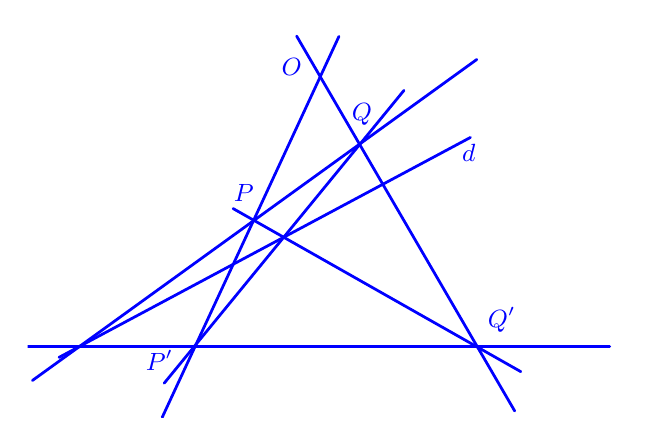
\begin{tikzpicture}[scale=1.5,line cap=round,line join=round,>=latex,x=1.0cm,y=1.0cm]
%\begin{axis}[x=1.0cm,y=1.0cm,axis lines=middle,ymajorgrids=true,xmajorgrids=true,
xmin=0,xmax=5,ymin=0,ymax=3.3,xtick={0,1,...,5},ytick={0,1,...,3},]
\clip(0,0) rectangle (5,3.3);
\draw [line width=1.pt,color=blue] (0.,0.6)-- (4.9286285963801575,0.6002813583766545);
\draw [line width=1.pt,color=blue] (1.1391070008551165,7.74681166972095E-4)-- (2.63536073107501,3.2258456183693847);
\draw [line width=1.pt,color=blue] (4.123658429164714,0.05421990115138969)-- (2.277262731210292,3.228641879813996);
\draw [line width=1.pt,color=blue] (0.2649933857468689,0.5081537857478451)-- (3.7487224149023524,2.370568589519966);
\draw [line width=1.pt,color=blue] (0.039993053225308196,0.3127145617204902)-- (3.8026584193723267,3.0307862309083062);
\draw [line width=1.pt,color=blue] (1.7392090953634105,1.7684996210059176)-- (4.175203589140998,0.38748192885109295);
\draw [line width=1.pt,color=blue] (1.1557522242512384,0.2897092179879971)-- (3.1860909833548168,2.769003408912047);
\begin{small}
%\draw [fill=blue] (2.47718913673507,2.884917738495868) circle (2.0pt);
\draw[color=blue] (2.23580887511578,2.967852412909658) node {$O$};
%\draw [fill=blue] (1.9134138174224284,1.6697392158264537) circle (2.0pt);
\draw[color=blue] (1.8298367808478124,1.8969260263062384) node {$P$};
%\draw [fill=blue] (2.8095991359765686,2.3134207356115613) circle (2.0pt);
\draw[color=blue] (2.8307679787843525,2.568879837508384) node {$Q$};
%\draw [fill=blue] (3.806080233595689,0.6002172759693696) circle (2.0pt);
\draw[color=blue] (4.0136866672548095,0.8259996397028188) node {$Q'$};
%\draw [fill=blue] (1.4171517891344274,0.6000809002989507) circle (2.0pt);
\draw[color=blue] (1.115885856445525,0.4830232152350569) node {$P'$};
%\draw [fill=blue] (3.7825997281286696,2.2453699209413687) circle (2.5pt);
\draw[color=blue] (3.7337059125872454,2.2378957149076465) node {$d$};
\end{small}
%\end{axis}
\end{tikzpicture}
\end{document} 